%--------------------------------------------------------------------
%导言区
% !Mode:: "TeX:UTF-8"

\documentclass[a4paper,UTF8]{ctexrep}
\let\cleardoublepage\clearpage

\usepackage{scuthesis}				% 封面版式
\usepackage{amssymb}  				% 设置数学公式
\usepackage{amsmath} 				% 设置数学公式编号
\usepackage{amsthm}					% 定理
\usepackage{booktabs}

%\usepackage[all,cmtip]{xy}			% xy-pic	画交换图
\usepackage{tikz}			        % tikz      绘图宏包
\usepackage{float}	  				% float		为固定图片位置宏包
\usepackage{subfigure}				% subfigure 引入宏包来添加多张图片 
\usepackage{caption}				% caption   为更改图片命名的宏包
\usepackage{enumerate}				% enumerate 有序列表环境
\usetikzlibrary{patterns,plotmarks}
%\usepackage{boondox-cal}			% boondox-cal   数学花体
%\usepackage{bm}       				% bm 			希腊字母加粗(普通字母类同)

\theoremstyle{plain}
	\newtheorem{thm}{定理~}[chapter]
	\newtheorem{lem}[thm]{引理~}
	\newtheorem{prop}[thm]{命题~}
	\newtheorem{cor}[thm]{推论~}
\theoremstyle{definition}
	\newtheorem{defn}[thm]{定义~}
	\newtheorem{conj}[thm]{猜想~}
	\newtheorem{exmp}[thm]{例~}
	\newtheorem{ques}[thm]{问题~}
	\newtheorem{rem}[thm]{注~}

%	该命令指定公式编号的格式
\numberwithin{equation}{chapter}
\renewcommand{\theequation}{\thechapter.\roman{equation}}

% 请在此处添加或修改你想要的定理样式,以下为英文定理样式,若使用中文写作请注释以下部分,并改用上面的中文定理样式(注意,使用英文写作时,若完成该操作后仍有部分单词显示为中文,请参照ctex文档第6节的“文档汉化”部分自行调整):
% \theoremstyle{plain}
%   \newtheorem{thm}{Theorem}[chapter]
%   \newtheorem{lem}[thm]{Lemma}
%   \newtheorem{prop}[thm]{Proposition}
%   \newtheorem{cor}[thm]{Corollary}
% \theoremstyle{definition}
%   \newtheorem{defn}[thm]{Definition}
%   \newtheorem{conj}[thm]{Conjecture}
%   \newtheorem{exmp}[thm]{Example}
%   \newtheorem{ques}[thm]{Question}
%   \newtheorem{rem}[thm]{Remark}
% \ctexset{bibname = {References}}
% \ctexset{proofname = {Proof}}
% \ctexset{contentsname = {Contents}}

%------------------------------------------------
	%基本信息
	\title{冷空气-蒸汽对流传热实验报告}
	\titleEng{Experimental Report of Cold air-steam convection heat transfer}
	
	\author{王诗煜}
	\authorEng{Shiyu Wang}
	\adviser{吴潘}
	\adviserEng{Pan Wu}
	
	\college{化学工程学院}
	\collegeEng{School of Chemical Engineering}
	\major{化学工程与工艺(虚拟的)}
	\majorEng{Chemical Engineering and Technics(virtual)}
	
	\grade{2023}
	\id{2022141500089}
	\date{\today}
	
 			% 作者信息


%-----------------------------------------------------------------
%正文区
	\begin{document}
	\zihao{-4}
	
	% 封面+摘要
	\makecover

\begin{abstract}{化工原理实验; 流体力学}
这一部分有意留白。
\end{abstract}


\begin{abstractEng}{Chemical Engineering Experiment; Fluid Mechaics}
This part intentionally left black.
\end{abstractEng}


\tableofcontents

        \chapter{报告正文}
	% 正文
	\section{实验目的}
	%----------------------------------------------
	\begin{enumerate}
            \item  观察⽓、液在填料塔内的操作状态,掌握吸收操作⽅法。
            \item  测定在不同喷淋量下,⽓体通过填料层的压降与⽓速的关系曲线。
	\end{enumerate}

        \section{实验原理}

        ⽓体混合物以⼀定⽓速通过填料塔内的填料层时,与吸收剂(液相)接触,进⾏物质传递。⽓、液两相在吸收塔内除了物质传递外,其流动相互影响,还具有⾃⼰的流体⼒学特性。填料塔的流体⼒学特性是吸收设备的重要参数,它包括了压降和液泛规律。测定填料塔的流体⼒学特性是了计算填料塔所需动⼒消耗和确定填料塔的适宜操作范围,选择适宜的⽓液负荷,也是确定最佳操作⽓速的依据。填料塔的流体⼒学特性以⽓体通过填料层所产⽣的压⼒降来表⽰。该压⼒降在填料因⼦、填料层⾼度、液体喷淋密度⼀定的情况下随⽓体速度的变化⽽变化。将气体压降与流速的关系绘制成双对数坐标图即可确定填料塔的流体⼒学特性。

        当气体流量增加到一定程度时,塔内填料或其他内部结构表面开始形成一层较薄的液膜,液体随气流在填料上分布,导致压降开始明显上升,这个临界气速就称为载点。载点反映的是系统开始进入较高气液负荷状态的起始阶段,是设计和运行时需要关注的拐点。

        随着气体流量进一步增加,液体的排出速度赶不上其在填料上的积累,导致填料或塔板上液体大量滞留,形成液泛现象。此时塔内压降会急剧增加,气流无法顺畅通过,整个系统趋于失稳,甚至出现泛塔的现象。泛点即为这种极限状态出现的气速,是操作时绝对不能达到的上限。

        \section{实验装置图及主要设备(包括名称、型号、规格)}

	 实验所使用的设备如下:
    
    
\begin{itemize}
    \item 内径为200mm,填料层高1m的填料塔以及配套的管路和夜罐
    \item 离心泵和离心风机
    \item 气体转子流量计
    \item 液体文丘里流量计
    \item 与管径相匹配的球阀和闸阀
    \item CS208-51C-A2SC型差压变送器
    \item 配套的控制系统
\end{itemize}
\newpage

本实验的装置图如下:


\begin{figure}[h]
    \centering
    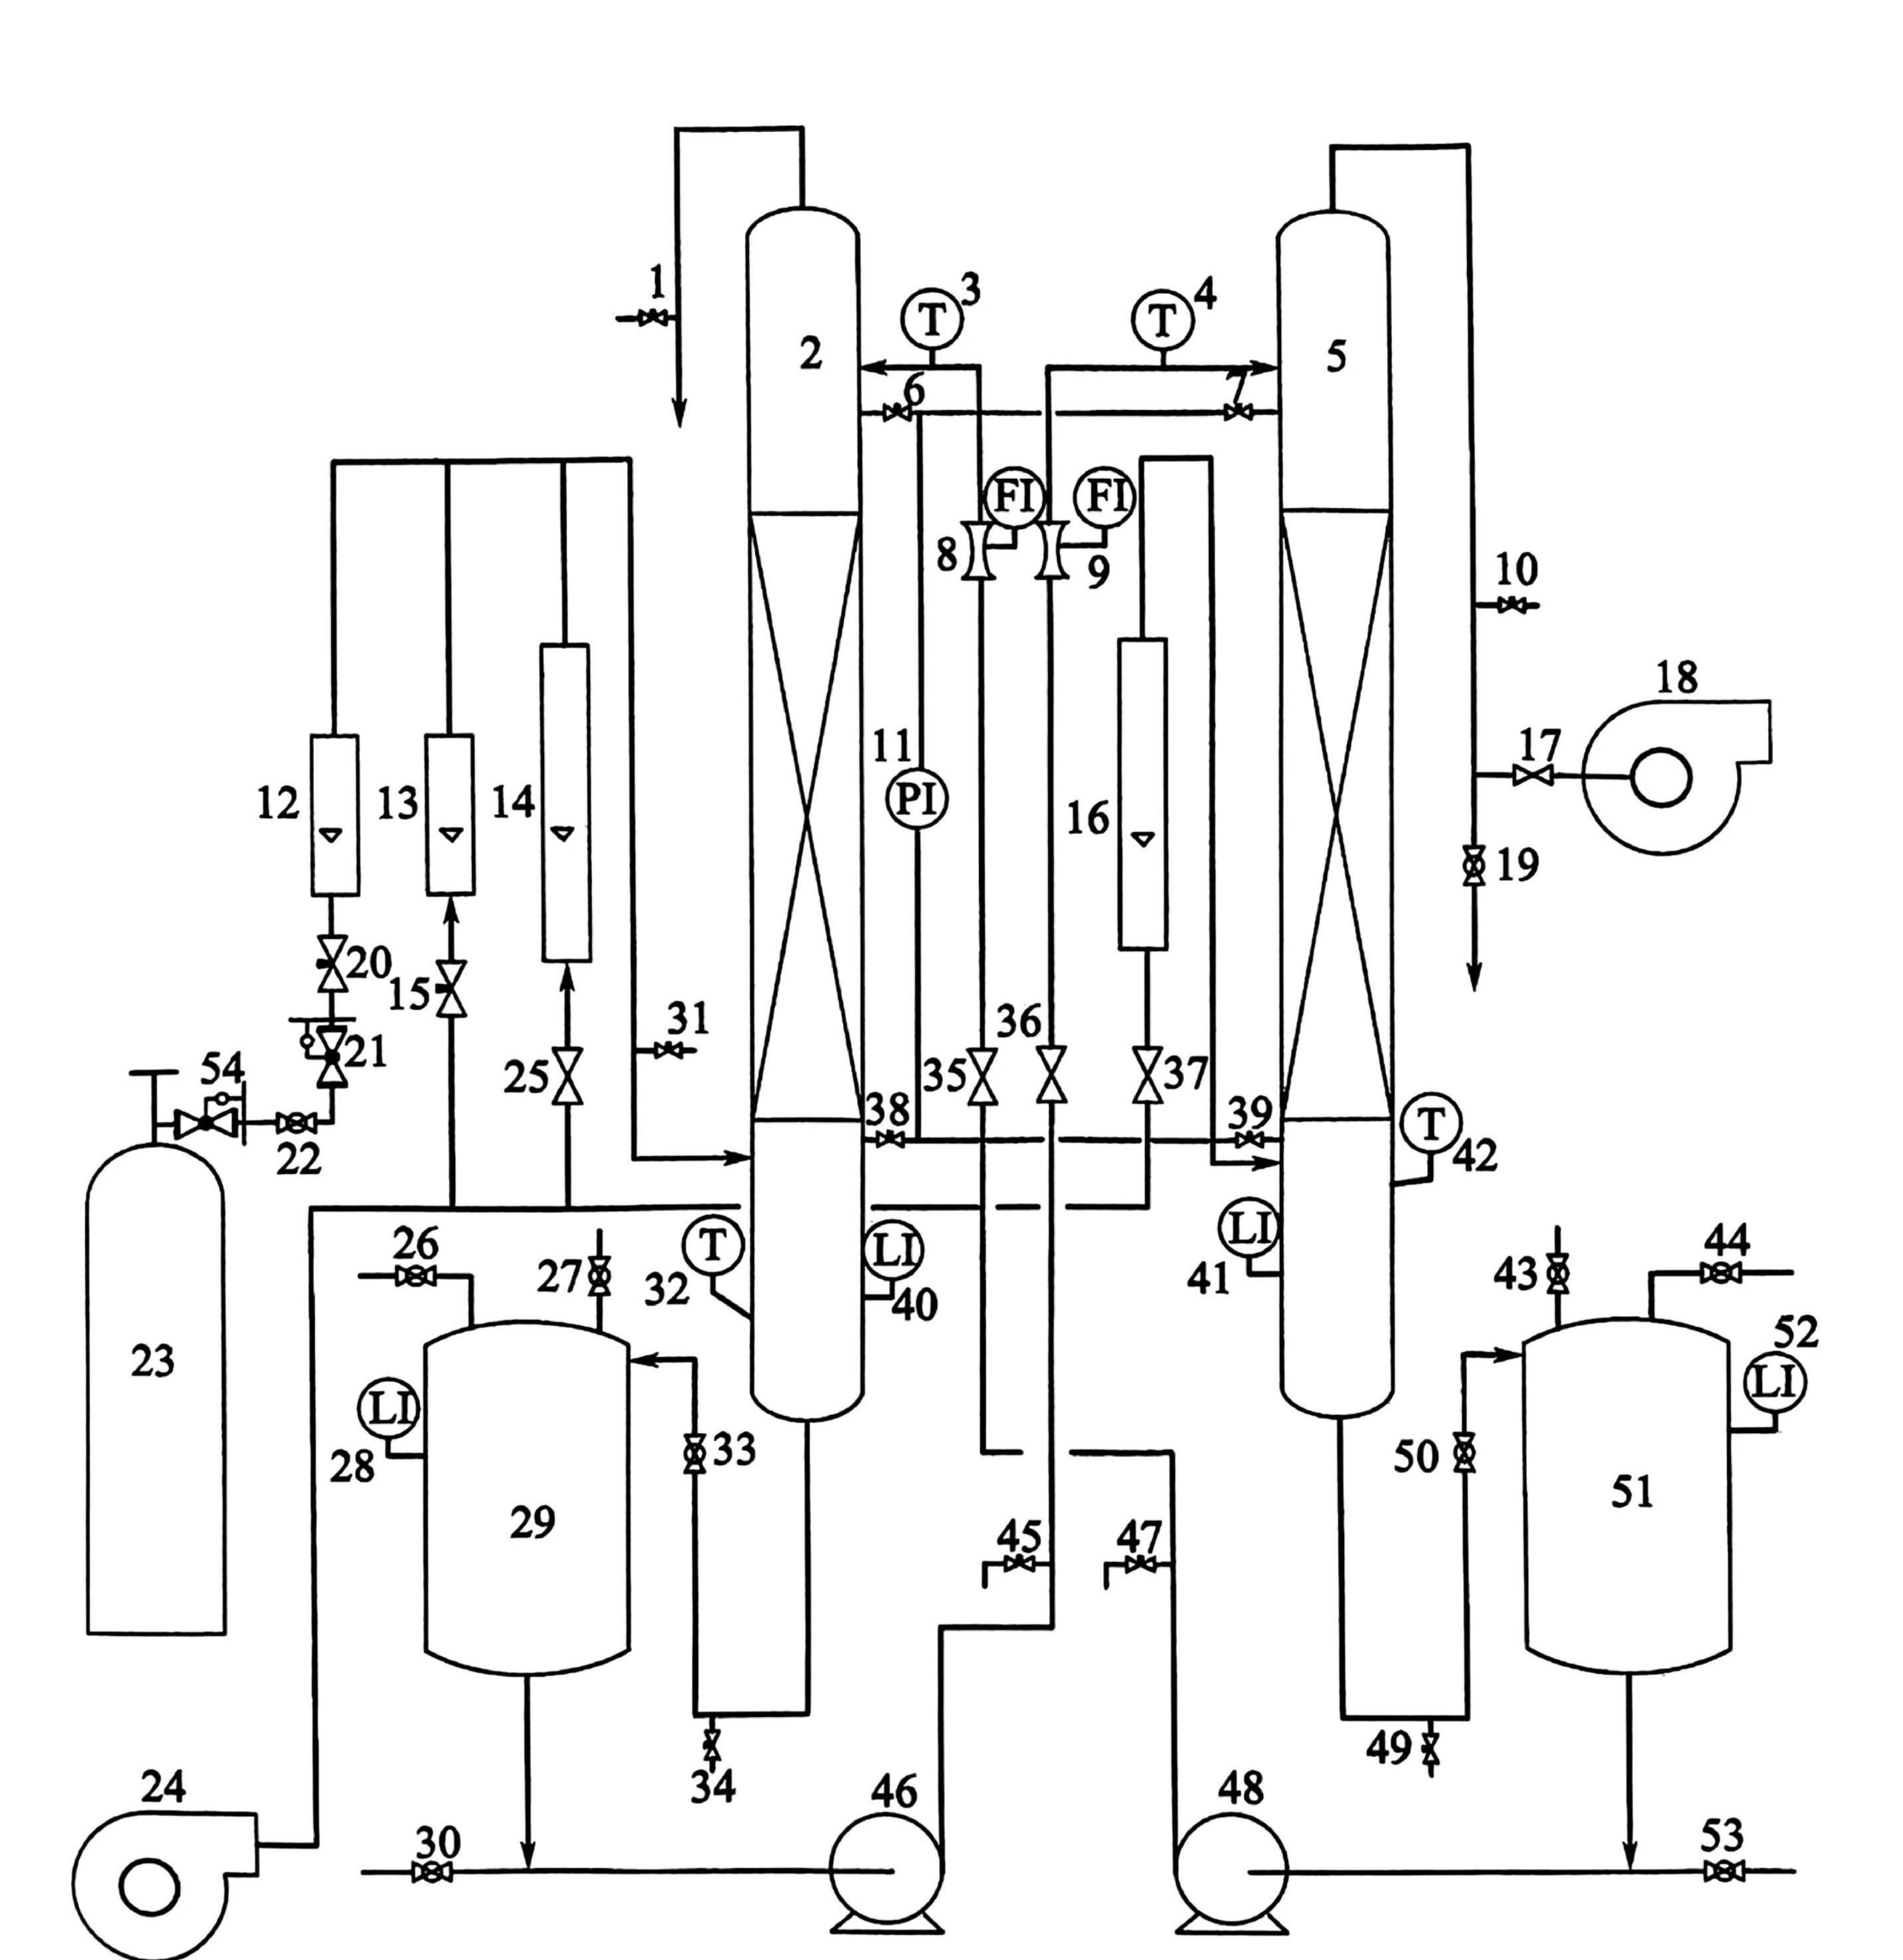
\includegraphics[width=0.7\linewidth]{吸收.pdf}
    \caption{本实验的装置示意图}
    \label{fig:enter-labesl}
\end{figure}

   

        \section{实验步骤}

        \begin{enumerate}
            \item 检查所有阀门是否处于关闭状态,检查夜罐液位是否正常,打开测压三通阀, 开启总电源与仪表电源。
            \item 关闭测压三通阀,启动风机,调节空⽓流量调节阀,让空⽓进⼊填料吸收塔底部,调节空⽓流量,流量从⼩到⼤,每调节⼀次风量,测定⼀次填料塔压降AP、转⼦流量计记录的空⽓流量V,共采集9组数据。
            \item 启动离心泵,通过闸阀或调节⽔量,保持吸收塔和解吸塔的喷淋量不变,注意观察⽔不能从塔顶尾⽓管内流出;⽤空⽓流量调节阀调节空⽓流量,流量从⼩到⼤,每调节⼀次风量,测定⼀次填料塔压降和转⼦流量计记录的空⽓流量,共采集7~10组数据
            \item 改变液流速,重复步骤3,从而测定不同⽔量下空塔⽓速与填料塔压降的变化曲线,完成⽓、液在填料塔内的流体⼒学性能测定。
        \end{enumerate}
\newpage
        \section{实验原始数据记录列表}
\begin{figure}[h]
    \centering
    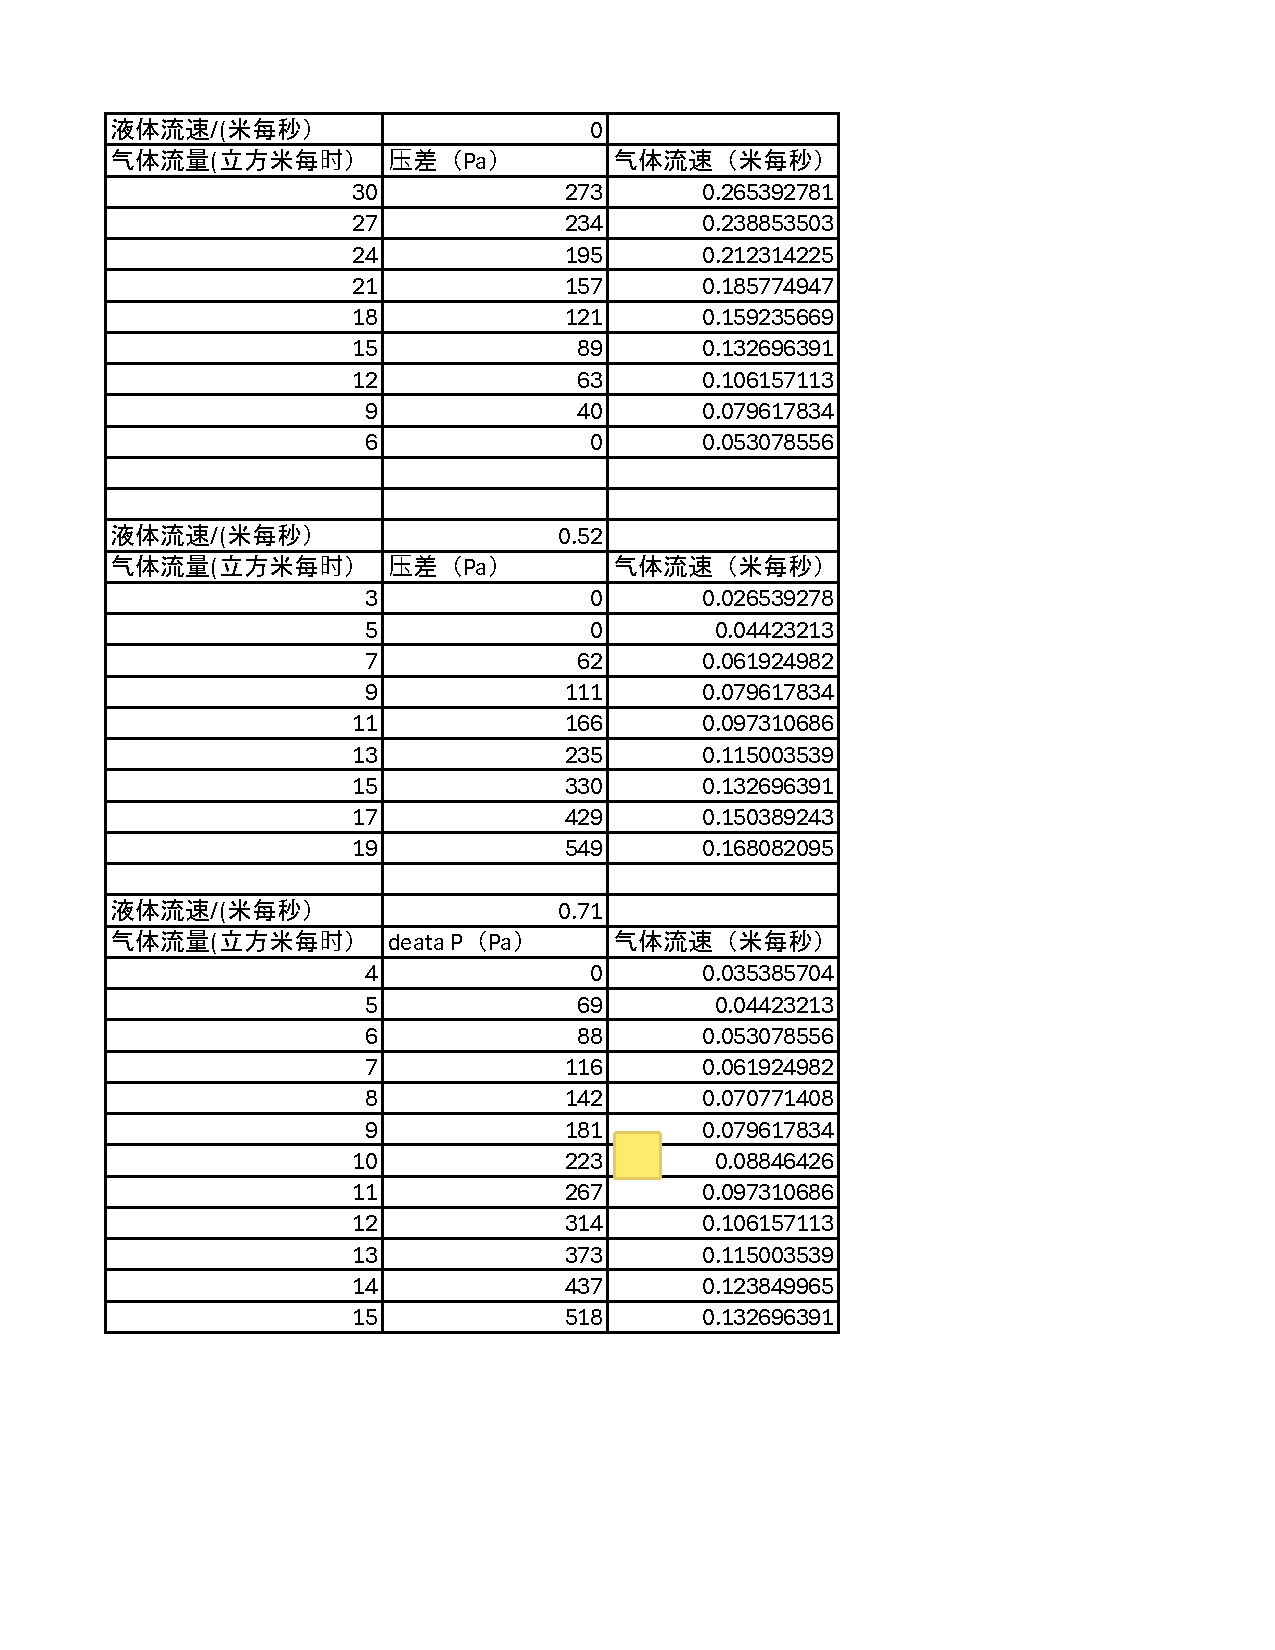
\includegraphics[width=0.8\linewidth]{Book1.pdf}
    \caption{本实验的原始数据}
    \label{fig:enter-lajsbel}
\end{figure}


        \section{实验数据处理(以一组实验数据为例进行计算)}
        在这里,我们需要在已知气体流量时求出塔内气体流速,这里以第一组数据为例。

        此时,$q_v=30m^3/h, d=200mm$将数据带入公式算出此时流速为:

        $$ u =\frac{q_v}{A^2}=\frac{4q_v}{\pi d^2}=0.27m/s$$


        用同样的方法可以算出其余组的气体流速。
        
        \section{实验结果、结论与分析}
\subsection{实验结果}
根据实验数据算出的不同液体流速下,气体流速与压差关系曲线如下:

\begin{figure}[h]
    \centering

\begin{tikzpicture}
\def\CheckTikzLibraryLoaded#1{ \ifcsname tikz@library@#1@loaded\endcsname \else \PackageWarning{tikz}{usetikzlibrary{#1} is missing in the preamble.} \fi }
\CheckTikzLibraryLoaded{patterns}
\CheckTikzLibraryLoaded{plotmarks}
\pgfdeclareplotmark{cross} {
\pgfpathmoveto{\pgfpoint{-0.3\pgfplotmarksize}{\pgfplotmarksize}}
\pgfpathlineto{\pgfpoint{+0.3\pgfplotmarksize}{\pgfplotmarksize}}
\pgfpathlineto{\pgfpoint{+0.3\pgfplotmarksize}{0.3\pgfplotmarksize}}
\pgfpathlineto{\pgfpoint{+1\pgfplotmarksize}{0.3\pgfplotmarksize}}
\pgfpathlineto{\pgfpoint{+1\pgfplotmarksize}{-0.3\pgfplotmarksize}}
\pgfpathlineto{\pgfpoint{+0.3\pgfplotmarksize}{-0.3\pgfplotmarksize}}
\pgfpathlineto{\pgfpoint{+0.3\pgfplotmarksize}{-1.\pgfplotmarksize}}
\pgfpathlineto{\pgfpoint{-0.3\pgfplotmarksize}{-1.\pgfplotmarksize}}
\pgfpathlineto{\pgfpoint{-0.3\pgfplotmarksize}{-0.3\pgfplotmarksize}}
\pgfpathlineto{\pgfpoint{-1.\pgfplotmarksize}{-0.3\pgfplotmarksize}}
\pgfpathlineto{\pgfpoint{-1.\pgfplotmarksize}{0.3\pgfplotmarksize}}
\pgfpathlineto{\pgfpoint{-0.3\pgfplotmarksize}{0.3\pgfplotmarksize}}
\pgfpathclose
\pgfusepathqstroke
}
\pgfdeclareplotmark{cross*} {
\pgfpathmoveto{\pgfpoint{-0.3\pgfplotmarksize}{\pgfplotmarksize}}
\pgfpathlineto{\pgfpoint{+0.3\pgfplotmarksize}{\pgfplotmarksize}}
\pgfpathlineto{\pgfpoint{+0.3\pgfplotmarksize}{0.3\pgfplotmarksize}}
\pgfpathlineto{\pgfpoint{+1\pgfplotmarksize}{0.3\pgfplotmarksize}}
\pgfpathlineto{\pgfpoint{+1\pgfplotmarksize}{-0.3\pgfplotmarksize}}
\pgfpathlineto{\pgfpoint{+0.3\pgfplotmarksize}{-0.3\pgfplotmarksize}}
\pgfpathlineto{\pgfpoint{+0.3\pgfplotmarksize}{-1.\pgfplotmarksize}}
\pgfpathlineto{\pgfpoint{-0.3\pgfplotmarksize}{-1.\pgfplotmarksize}}
\pgfpathlineto{\pgfpoint{-0.3\pgfplotmarksize}{-0.3\pgfplotmarksize}}
\pgfpathlineto{\pgfpoint{-1.\pgfplotmarksize}{-0.3\pgfplotmarksize}}
\pgfpathlineto{\pgfpoint{-1.\pgfplotmarksize}{0.3\pgfplotmarksize}}
\pgfpathlineto{\pgfpoint{-0.3\pgfplotmarksize}{0.3\pgfplotmarksize}}
\pgfpathclose
\pgfusepathqfillstroke
}
\pgfdeclareplotmark{newstar} {
\pgfpathmoveto{\pgfqpoint{0pt}{\pgfplotmarksize}}
\pgfpathlineto{\pgfqpointpolar{44}{0.5\pgfplotmarksize}}
\pgfpathlineto{\pgfqpointpolar{18}{\pgfplotmarksize}}
\pgfpathlineto{\pgfqpointpolar{-20}{0.5\pgfplotmarksize}}
\pgfpathlineto{\pgfqpointpolar{-54}{\pgfplotmarksize}}
\pgfpathlineto{\pgfqpointpolar{-90}{0.5\pgfplotmarksize}}
\pgfpathlineto{\pgfqpointpolar{234}{\pgfplotmarksize}}
\pgfpathlineto{\pgfqpointpolar{198}{0.5\pgfplotmarksize}}
\pgfpathlineto{\pgfqpointpolar{162}{\pgfplotmarksize}}
\pgfpathlineto{\pgfqpointpolar{134}{0.5\pgfplotmarksize}}
\pgfpathclose
\pgfusepathqstroke
}
\pgfdeclareplotmark{newstar*} {
\pgfpathmoveto{\pgfqpoint{0pt}{\pgfplotmarksize}}
\pgfpathlineto{\pgfqpointpolar{44}{0.5\pgfplotmarksize}}
\pgfpathlineto{\pgfqpointpolar{18}{\pgfplotmarksize}}
\pgfpathlineto{\pgfqpointpolar{-20}{0.5\pgfplotmarksize}}
\pgfpathlineto{\pgfqpointpolar{-54}{\pgfplotmarksize}}
\pgfpathlineto{\pgfqpointpolar{-90}{0.5\pgfplotmarksize}}
\pgfpathlineto{\pgfqpointpolar{234}{\pgfplotmarksize}}
\pgfpathlineto{\pgfqpointpolar{198}{0.5\pgfplotmarksize}}
\pgfpathlineto{\pgfqpointpolar{162}{\pgfplotmarksize}}
\pgfpathlineto{\pgfqpointpolar{134}{0.5\pgfplotmarksize}}
\pgfpathclose
\pgfusepathqfillstroke
}
\definecolor{c}{rgb}{1,1,1};
\draw [color=c, fill=c] (0,0) rectangle (20,14.411);
\draw [color=c, fill=c] (2.03008,1.4411) rectangle (18.0201,12.9449);
\definecolor{c}{rgb}{0,0,0};
\draw [c,line width=0.9] (2.03008,1.4411) -- (2.03008,12.9449) -- (18.0201,12.9449) -- (18.0201,1.4411) -- (2.03008,1.4411);
\definecolor{c}{rgb}{1,1,1};
\draw [color=c, fill=c] (2.03008,1.4411) rectangle (18.0201,12.9449);
\definecolor{c}{rgb}{0,0,0};
\draw [c,line width=0.9] (2.03008,1.4411) -- (2.03008,12.9449) -- (18.0201,12.9449) -- (18.0201,1.4411) -- (2.03008,1.4411);
\draw [c,line width=0.9] (2.03008,1.4411) -- (18.0201,1.4411);
\draw [c,line width=0.9] (3.44118,1.61393) -- (3.44118,1.4411);
\draw [c,line width=0.9] (5.12402,1.61393) -- (5.12402,1.4411);
\draw [c,line width=0.9] (6.499,1.61393) -- (6.499,1.4411);
\draw [c,line width=0.9] (7.66152,1.61393) -- (7.66152,1.4411);
\draw [c,line width=0.9] (8.66855,1.61393) -- (8.66855,1.4411);
\draw [c,line width=0.9] (9.55681,1.61393) -- (9.55681,1.4411);
\draw [c,line width=0.9] (10.3514,1.78675) -- (10.3514,1.4411);
\draw [anchor=base] (10.3514,0.789004) node[scale=1.11327, color=c, rotate=0]{$10^{-1}$};
\draw [c,line width=0.9] (15.5788,1.61393) -- (15.5788,1.4411);
\draw [anchor= east] (18.0201,0.634085) node[scale=1.11327, color=c, rotate=0]{ gas flow rate/(m/s)};
\draw [c,line width=0.9] (2.03008,1.4411) -- (2.03008,12.9449);
\draw [c,line width=0.9] (2.26955,2.01234) -- (2.03008,2.01234);
\draw [c,line width=0.9] (2.26955,3.02301) -- (2.03008,3.02301);
\draw [c,line width=0.9] (2.26955,3.80695) -- (2.03008,3.80695);
\draw [c,line width=0.9] (2.26955,4.44747) -- (2.03008,4.44747);
\draw [c,line width=0.9] (2.26955,4.98903) -- (2.03008,4.98903);
\draw [c,line width=0.9] (2.26955,5.45814) -- (2.03008,5.45814);
\draw [c,line width=0.9] (2.26955,5.87193) -- (2.03008,5.87193);
\draw [c,line width=0.9] (2.50903,6.24208) -- (2.03008,6.24208);
\draw [anchor= east] (1.87407,6.24208) node[scale=1.11327, color=c, rotate=0]{$10^{2}$};
\draw [c,line width=0.9] (2.26955,8.67721) -- (2.03008,8.67721);
\draw [c,line width=0.9] (2.26955,10.1017) -- (2.03008,10.1017);
\draw [c,line width=0.9] (2.26955,11.1123) -- (2.03008,11.1123);
\draw [c,line width=0.9] (2.26955,11.8963) -- (2.03008,11.8963);
\draw [c,line width=0.9] (2.26955,12.5368) -- (2.03008,12.5368);
\draw [anchor= east] (0.678446,12.9449) node[scale=1.11327, color=c, rotate=90]{pressure drop/(Pa)};
\definecolor{c}{rgb}{1,0,0};
\draw [c,line width=1.8] (17.7122,9.77035) -- (16.9176,9.22879) -- (16.0294,8.58827) -- (15.0223,7.82678) -- (13.8598,6.91176) -- (12.4848,5.83268) -- (10.802,4.61888) -- (8.63243,3.02302);
\foreach \P in {(17.7122,9.77035), (16.9176,9.22879), (16.0294,8.58827), (15.0223,7.82678), (13.8598,6.91176), (12.4848,5.83268), (10.802,4.61888), (8.63243,3.02302)}{\draw[mark options={color=c,fill=c},mark size=3.603604pt, line width=0.000000pt,
 mark=*] plot coordinates {\P};}
\definecolor{c}{rgb}{0,0,1};
\draw [c,line width=1.8] (6.73714,4.56267) -- (8.63243,6.60872) -- (10.1458,8.02261) -- (11.4056,9.24378) -- (12.4848,10.4365) -- (13.4287,11.3582) -- (14.2675,12.2247);
\foreach \P in {(6.73714,4.56267), (8.63243,6.60872), (10.1458,8.02261), (11.4056,9.24378), (12.4848,10.4365), (13.4287,11.3582), (14.2675,12.2247)}{\draw[mark options={color=c,fill=c},mark size=3.603604pt, line width=0.000000pt, mark=square*] plot
 coordinates {\P};}
\definecolor{c}{rgb}{0,1,0};
\draw [c,line width=1.8] (4.19963,4.93848) -- (5.57461,5.79299) -- (6.73714,6.76351) -- (7.74416,7.474) -- (8.63243,8.32653) -- (9.427,9.05964) -- (10.1458,9.69228) -- (10.802,10.2619) -- (11.4056,10.8668) -- (11.9645,11.4232) -- (12.4848,12.0205);
\foreach \P in {(4.19963,4.93848), (5.57461,5.79299), (6.73714,6.76351), (7.74416,7.474), (8.63243,8.32653), (9.427,9.05964), (10.1458,9.69228), (10.802,10.2619), (11.4056,10.8668), (11.9645,11.4232), (12.4848,12.0205)}{\draw[mark
 options={color=c,fill=c},mark size=3.603604pt, line width=0.000000pt, mark=triangle*] plot coordinates {\P};}
\definecolor{c}{rgb}{1,1,1};
\draw [color=c, fill=c] (3.08271,9.97494) rectangle (7.06767,12.8822);
\definecolor{c}{rgb}{0,0,0};
\draw [c,line width=0.9] (3.08271,9.97494) -- (7.06767,9.97494);
\draw [c,line width=0.9] (7.06767,9.97494) -- (7.06767,12.8822);
\draw [c,line width=0.9] (7.06767,12.8822) -- (3.08271,12.8822);
\draw [c,line width=0.9] (3.08271,12.8822) -- (3.08271,9.97494);
\draw [anchor= west] (4.07895,12.3977) node[scale=1.00194, color=c, rotate=0]{V=0 (m/s)};
\definecolor{c}{rgb}{1,0,0};
\draw [c,line width=1.8] (3.23214,12.3977) -- (3.92951,12.3977);
\definecolor{c}{rgb}{0,0,0};
\draw [anchor= west] (4.07895,11.4286) node[scale=1.00194, color=c, rotate=0]{V=0.5 (m/s)};
\definecolor{c}{rgb}{0,0,1};
\draw [c,line width=1.8] (3.23214,11.4286) -- (3.92951,11.4286);
\definecolor{c}{rgb}{0,0,0};
\draw [anchor= west] (4.07895,10.4595) node[scale=1.00194, color=c, rotate=0]{V=0.7 (m/s)};
\definecolor{c}{rgb}{0,1,0};
\draw [c,line width=1.8] (3.23214,10.4595) -- (3.92951,10.4595);
\definecolor{c}{rgb}{0,0,0};
\draw (10,13.9179) node[scale=1.00194, color=c, rotate=0]{Relationship between gas flow rate and pressure drop in packed tower};
\end{tikzpicture}
    \caption{填料塔气体流速与压降关系}
    \label{fig:enter-label}
\end{figure}


\subsection{实验结果分析与结论}

根据画出的关系图,在不同的液体流速下,气体经过填料塔的压降与气体流速的关系图在双对数坐标图下均成直线,且不同液体流速下的图像几乎平行。虽然在实验中观察到了液泛的现象但图中并没有出现的泛点。
经过分析,没有出现泛点的原因可能是实验中存在偏流使得气体和液体分布不均,从而导致泛点不明显。并且在出现泛点后为了放置泛塔而读数过早,导致没有记录到压差增大的现象。


        \section{实验思考题}
	1.填料吸收塔塔底为什么有液封装置?采⽤了什么原理进⾏液封? 

    答:填料吸收塔的塔底设置液封装置的主要目的是防止气体倒流、维持塔内稳定操作,并确保气液相合理分布。液封的原理主要基于液柱静压力平衡,即通过液体形成的静压力防止气体进入或逸出非期望的通道。

    2.在填料塔的流体⼒学特性中,确定的最佳操作空塔⽓速是多少?
    
    答:一般来说,泛点气速的0.6~0.8倍为最佳空塔气速。本实验中并没有测出泛点气速,所以还无法确定最佳的空塔气速。

	
	% 后记(附录)
	%%----------------------------------------------
%	附录Appendix
\appendix{
			\chapter{数据处理所涉及的代码或操作}
   \section{Python 代码}
\begin{lstlisting}[language= Python]
import numpy as np
import scipy as sp

\end{lstlisting}

\section{Origin 操作}
\begin{enumerate}
    \item 打开软件
\end{enumerate}
}
	
	\appendix{
			\chapter{绘图所用到的代码}
\begin{lstlisting}[language= C++]
#include <Eigen/Dense>
#include <Eigen/src/Core/GlobalFunctions.h>
#include <Eigen/src/Core/Matrix.h>
#include <TApplication.h>
#include <TAxis.h>
#include <TCanvas.h>
#include <TGraph.h>
#include <TLatex.h>
#include <TLegend.h>
#include <TMultiGraph.h>
#include <cmath>
#include <cstdio>
#include <cstdlib>
#include <iostream>
#include <numbers>
#include <openblas/cblas.h>
#include <openblas/openblas_config.h>
#include <openblas_config.h>
#include <torch/torch.h>
#include <vector>

using namespace std;
using namespace Eigen;

void draw_loglog_plot() {
  // 创建 Canvas
  TCanvas *c1 = new TCanvas("c1", "Log-Log Plot", 800, 600);

  // 设置对数坐标
  c1->SetLogx();
  c1->SetLogy();

  // 创建多个 TGraph 数据集
  double x1[] = {0.265392781, 0.238853503, 0.212314225,
                 0.185774947, 0.159235669, 0.132696391,
                 0.106157113, 0.079617834};
  double y1[] = {273, 234, 195, 157, 121, 89, 63, 40};
  TGraph *gr1 = new TGraph(8, x1, y1);
  gr1->SetLineColor(kRed);
  gr1->SetLineWidth(2);
  gr1->SetTitle("V=0");
  gr1->SetMarkerStyle(20); // 圆形
  gr1->SetMarkerSize(1.5);
  gr1->SetMarkerColor(kRed);

  double x2[] = {0.061924982,
                 0.079617834, 0.097310686, 0.115003539,
                 0.132696391, 0.150389243, 0.168082095};
  double y2[] = {62, 111, 166, 235, 330, 429, 549};
  TGraph *gr2 = new TGraph(7, x2, y2);
  gr2->SetLineColor(kBlue);
  gr2->SetLineWidth(2);
  gr2->SetTitle("V=0.5");
  gr2->SetMarkerStyle(21); // 圆形
  gr2->SetMarkerSize(1.5);
  gr2->SetMarkerColor(kBlue);

  double x3[] = {0.04423213,  0.053078556, 0.061924982,
                 0.070771408, 0.079617834, 0.08846426,  0.097310686,
                 0.106157113, 0.115003539, 0.123849965, 0.132696391};
  double y3[] = {69, 88, 116, 142, 181, 223, 267, 314, 373, 437, 518};
  TGraph *gr3 = new TGraph(11, x3, y3);
  gr3->SetLineColor(kGreen);
  gr3->SetLineWidth(2);
  gr3->SetTitle("V=0.7");
  gr3->SetMarkerStyle(22); // 圆形
  gr3->SetMarkerSize(1.5);
  gr3->SetMarkerColor(kGreen);

  TLatex latex;
  latex.SetTextFont(43);

  // 使用 TMultiGraph 组合多个数据集
  TMultiGraph *mg = new TMultiGraph();
  mg->Add(gr1);
  mg->Add(gr2);
  mg->Add(gr3);
  mg->SetTitle("Relationship between gas flow rate and pressure drop in packed "
               "tower; gas flow rate/(m/s);pressure drop/(Pa)");

  // 绘制
  mg->Draw("APL");

  // 添加图例
  TLegend *leg = new TLegend(0.7, 0.7, 0.9, 0.9);
  leg->AddEntry(gr1, "V=0 (m/s)", "l");

  leg->AddEntry(gr2, "V=0.5 (m/s)", "l");
  leg->AddEntry(gr3, "V=0.7 (m/s)", "l");
  leg->SetTextFont(43); // 43 表示支持 Unicode 字体
  leg->SetTextSize(18); // 设置字体大小
  leg->Draw();

  // 显示 Canvas
  c1->Update();
  // c1->SaveAs("loglog_plot.png"); // 可选:保存图像
}

int main(int argc, char **argv) {
  TApplication app("ROOT Application", &argc, argv);
  draw_loglog_plot();
  app.Run(); // 进入 ROOT 事件循环,保持窗口打开
  return 0;
}
\end{lstlisting}
}
	% 参考文献
	%\addcontentsline{toc}{chapter}{参考文献}			% 在目录中添加参考文献
	%\bibliographystyle{unsrt}
	%\bibliography{ref/refs}
	
	% 声明
        \addcontentsline{toc}{chapter}{声\hspace{0.8cm}明}
	\section*{声\hspace{0.8cm}明}


%-------------------------------------------------------------------
	本人声明所呈交的实验报告是本人在教师指导下进行的实验工作及取得的实验成果。据我所知,除了文中特别加以标注和致谢的地方外,报告中不包含其他人已经发表或撰写过的成果,也不包含为获得四川大学或其他教育机构的学位或证书而使用过的材料。与我一同工作的同志对本实验所做的任何贡献均已在中作了明确的说明并表示谢意。
	
	本实验报告成果是本人在四川大学修读课程化工原理及仿真实验期间在教师指导下取得的,报告没有所有权归属。任何组织或个人被允许以任何合法目的,在不取得任何许可的情况下使用此报告中的部分或全部内容且需要承担由此引发的全部后果,特此声明。
	
	\vspace{40pt}
	\begin{flushright}
		\begin{tabular}{b{4cm} >{\centering\arraybackslash}b{2.5cm} }
			\songti \zihao{-4} 实验报告作者(签名)& {} \\[-3pt] 
			\cline{2-2} \\ [0.6cm]
                \songti \zihao{-4} 报告指导教师(签名)& {} \\[-3pt] 
			\cline{2-2} \\ [0.6cm]
		\end{tabular}
		
		\today
	\end{flushright}
	
	

	
	
\end{document} 
	
